\chapter*{Introduction}
\addcontentsline{toc}{chapter}{Introduction}
\chaptermark{Introduction}

% Essor de l'IA
L'intelligence artificielle (IA) est aujourd'hui partout dans nos quotidiens. Les modèles complexes tels que les réseaux de neurones sont notamment utilisés pour traiter automatiquement les textes qui nous entourent.
% Inexplicable
La figure~\ref{fig:ratio_perf_explicabilite} présente différentes solutions d'intelligence artificielle. Elle met en avant la corrélation entre meilleures performantes et explicabilité décroissante.
De bas en haut, les solutions sont de plus en plus performantes; on retrouve alors les trois ères de l'IA. La première période des années 1960 est celle des systèmes experts ou ``la bonne vieille IA'' (\textit{Good Old Fashioned AI}, \textit{GOFAI}), avec des systèmes tels qu'ELIZA~\cite{Weizenbaum1966}.
Vient ensuite celle de l'apprentissage automatique avec des systèmes simples tels que les régressions linéaires. %, jusqu'aux systèmes ensemblistes comprenant les forêts aléatoires.
Enfin, l'avènement de l'apprentissage profond a contribué à l'entraînement de modèles complexes, résolvant des problèmes pointus~\cite{LeCun2015}.
% ce qui implique des problemes
Ce manque d'explicabilité est un problème auquel s'intéressent les communautés scientifique et industrielle.
% chart rapport complexité - explicabilité
\begin{figure}[htpb!]
    \centering
    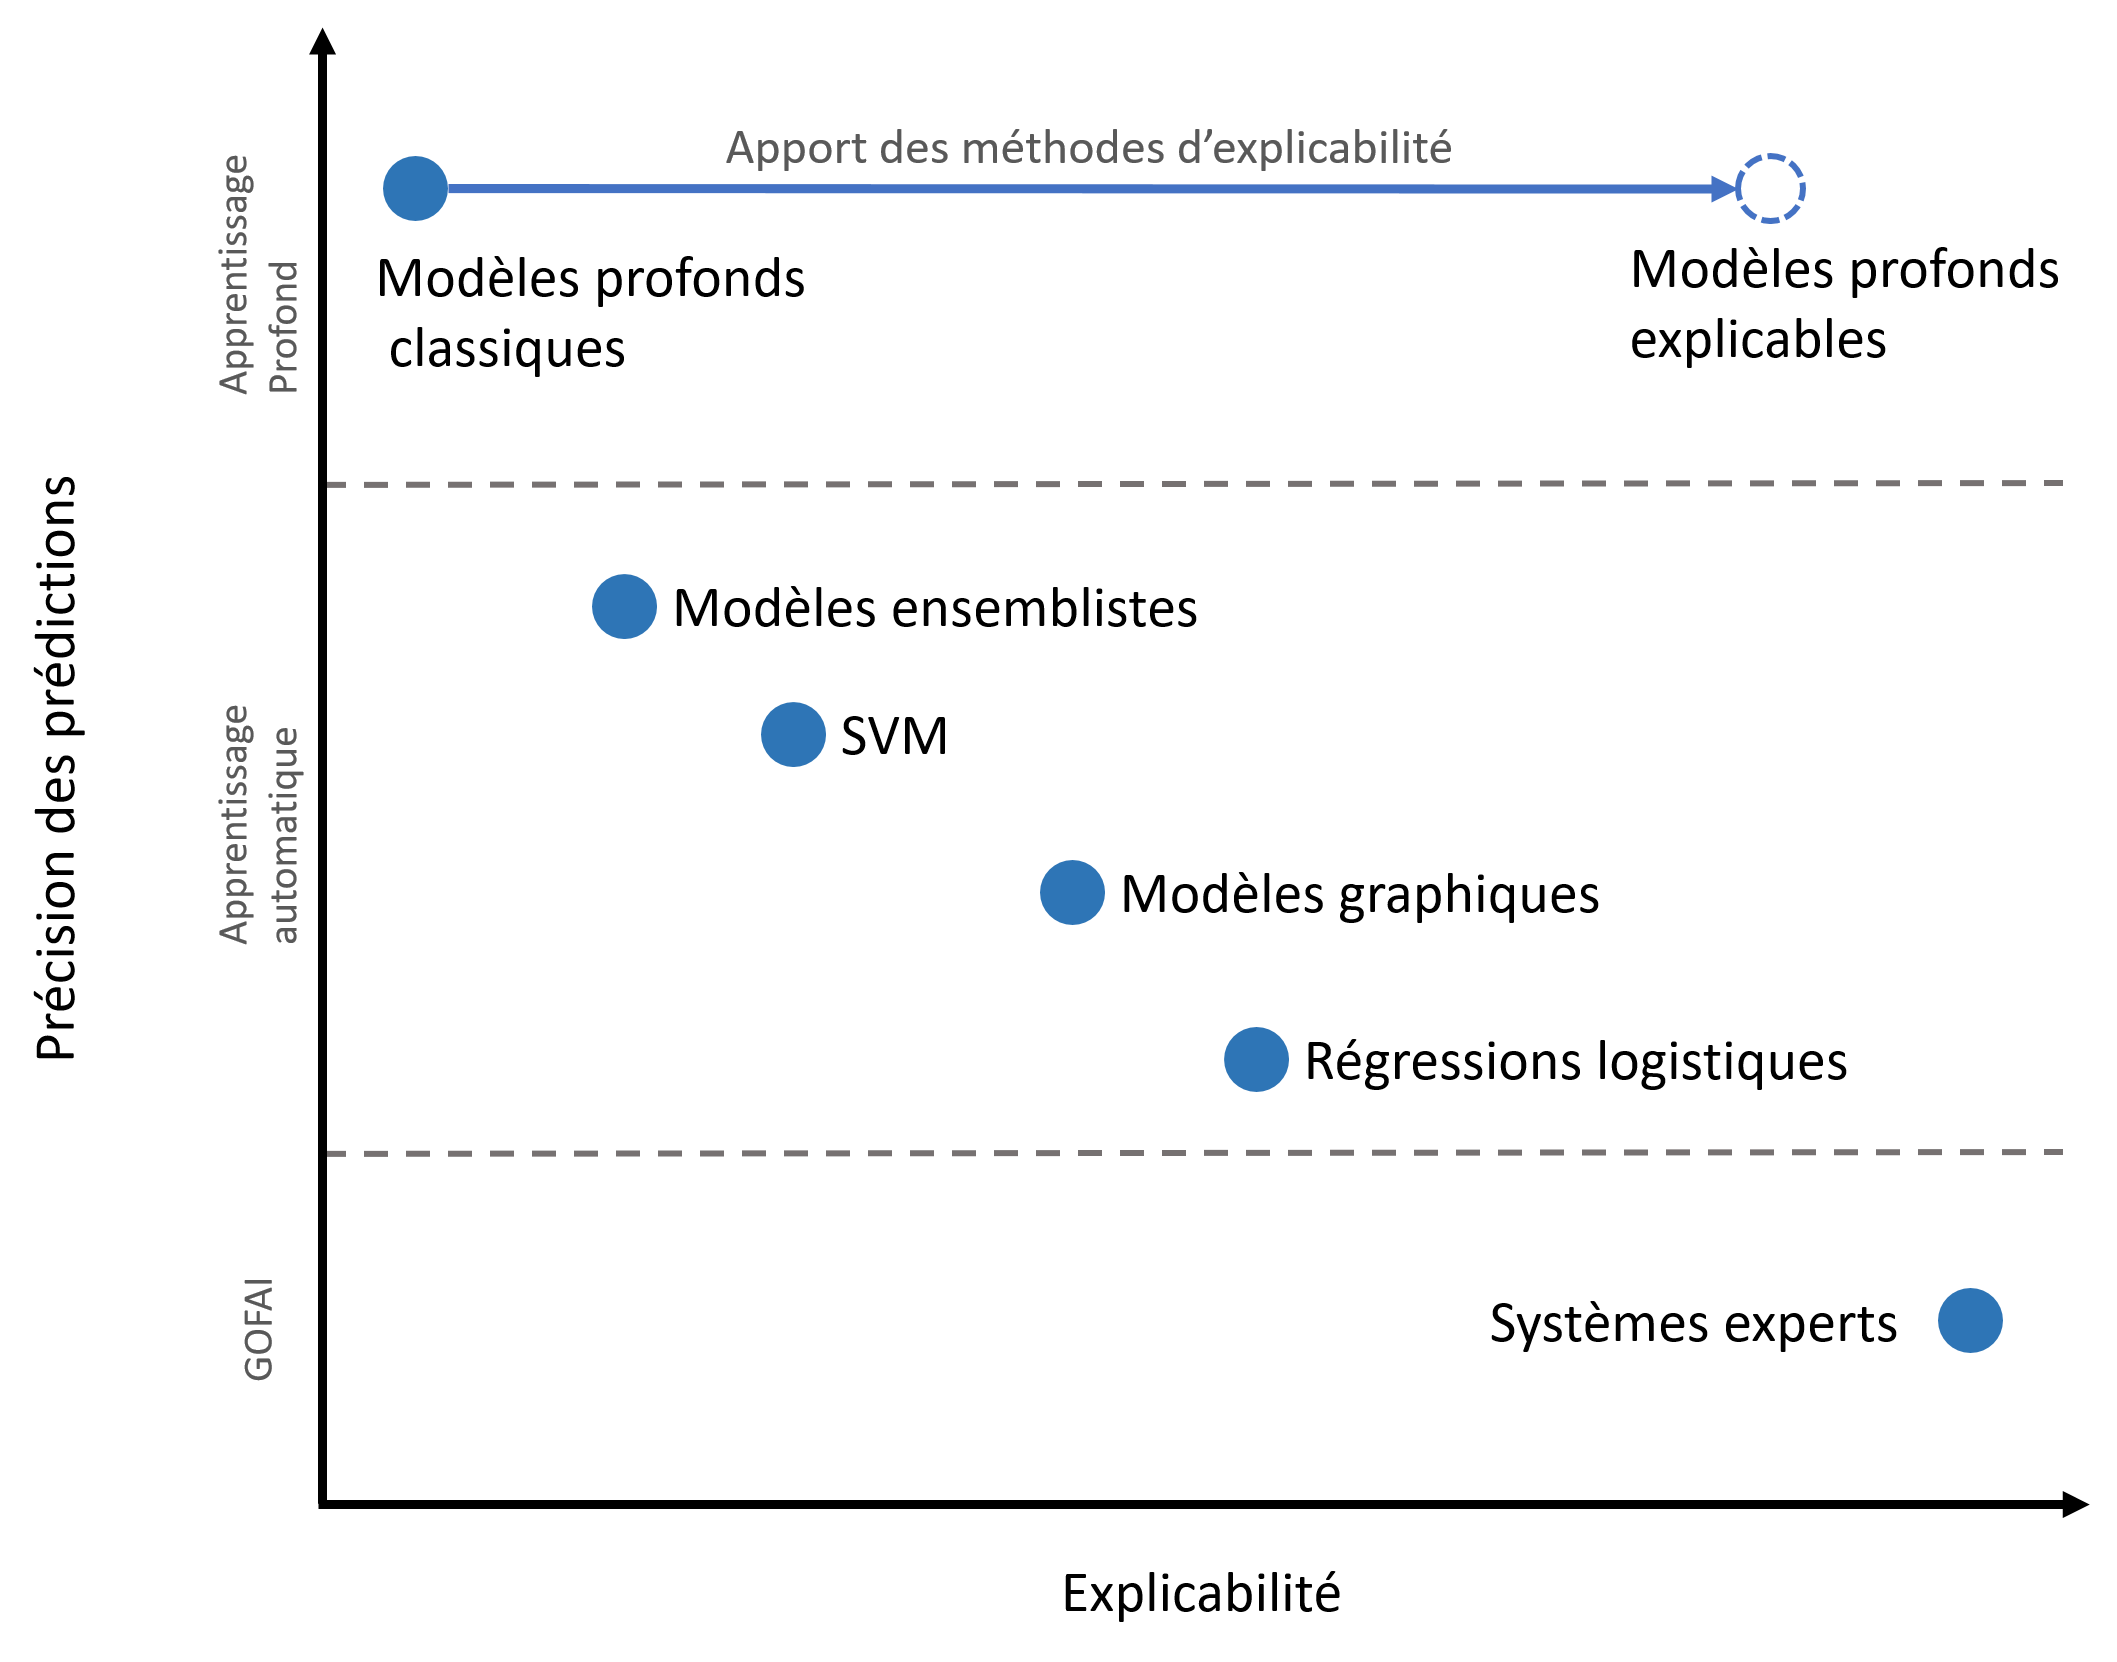
\includegraphics[width=0.78\textwidth]{Introduction/figures/performance_explicabilite.png}
    \caption{Différentes familles de solutions d'intelligence artificielle, selon leur précision de prédiction, et leur explicabilité. Figure inspirée de \cite{Dam2018}.}
    \label{fig:ratio_perf_explicabilite}
\end{figure}

\paragraph{L'explicabilité} est la capacité d'un système à être compris par un humain étant donné un contexte. L'explication peut prendre diverses formes et s'adapter à son receveur. % rappel différence avec transparence, interprétabilité
Les informations brutes comme le code source d'un algorithme ou la structure d'un modèle ne sont pas des explications mais de la transparence. Celle-ci ne suffit pas à rendre un modèle explicable, surtout si ce dernier est complexe.

% Pour les scientifiques
\paragraph{Pour la communauté scientifique} la performance des modèles a longtemps été mesurée par des scores de prédiction : précision, rappel, F1-score permettent les comparatifs de modèles d'IA.
Toutefois, les scores faibles n'indiquent pas les faiblesses d'un modèle. Le développement de ces modèles est alors contraint aux essais-erreurs.
On pourrait se contenter de modèles très performants. %La confiance obtenue grâce à de bons résultats ne suffit-elle pas ?
\cite{Dam2018} dit que les explications sont nécessaires quand les résultats d'un modèle ne correspondent pas aux suppositions des utilisateurs.
Pourtant, un modèle avec de bonnes prédictions peut les effectuer pour de mauvaises raisons. %Ainsi dans~\cite{Ribeiro2016}, les auteurs présentent un modèle devant différencier des images de loups et de huskys, qui en réalité a appris à différencier les images présentant de la neige ou non en arrière-plan.
% notion d'accountability
Le domaine de l'Intelligence Artificielle Explicable (XAI) est aujourd'hui en plein essor. L'explicabilité permet d'améliorer un modèle, ainsi que son adoption par les utilisateurs.

% Et l'industrie
\paragraph{Pour l'industrie et les services publics} l'explicabilité est également importante. Un manque d'acceptabilité freinera l'adoption d'outils, tandis qu'une confiance totale rendra difficile la détection de dysfonctionnements d'un modèle d'IA. Cette problématique est d'autant plus présente dans des domaines tels que la conduite autonome, les soins médicaux, et l'accompagnement des personnes.
Le besoin de transparence et d'explications est également transcrit dans les législations~\cite{DoshiVelez2017a,Desmoulin2019}.
Ainsi le Règlement Général sur la Protection des Données (RGPD)~\cite{Commission2018} indique que tout traitement de données personnelles des citoyens et citoyennes européennes doit être communiqué de manière accessible, en langage clair et net. Toutefois, cette contrainte juridique est aujourd'hui limitée~\cite{Wachter2017}.
%  \begin{quote} % 39 :
%  \textit{The principle of transparency requires that any information and communication relating to the processing of those personal data be easily accessible and easy to understand, and that clear and plain language be used.}
% \end{quote}
La loi pour une république numérique~\cite{Legifrance2016} exige quant à elle que les traitements concernant un usager en particulier, soient communiqués sur demande de ce dernier. % Son cadre d'application est en revanche restreint aux organismes publics français.
% \begin{quote}
%     Une décision individuelle prise sur le fondement d'un traitement algorithmique comporte une mention explicite en informant l'intéressé. Les règles définissant ce traitement ainsi que les principales caractéristiques de sa mise en œuvre sont communiquées par l'administration à l'intéressé s'il en fait la demande.
% \end{quote}
La question se pose alors de trouver le bon compromis entre la performance du modèle et son explicabilité.

\section*{Contributions}
\addcontentsline{toc}{section}{Contribution}
% traiter chaque mot de mon sujet
L'objectif de la thèse est de rendre plus explicables les modèles profonds permettant de traiter des textes.
La figure \ref{fig:environnement} présente l'environnement de notre contribution. Des utilisateurs veulent rendre un service ou bénéficier d'un service. Iels vont pour cela utiliser un outil, lequel peut appeler un modèle pour obtenir le résultat d'une prédiction, classification ou recommandation. Ce modèle complexe est issu d'un entraînement défini par un algorithme et un large ensemble de données, dans notre cas des textes.

\begin{figure}[htpb!]
    \centering
    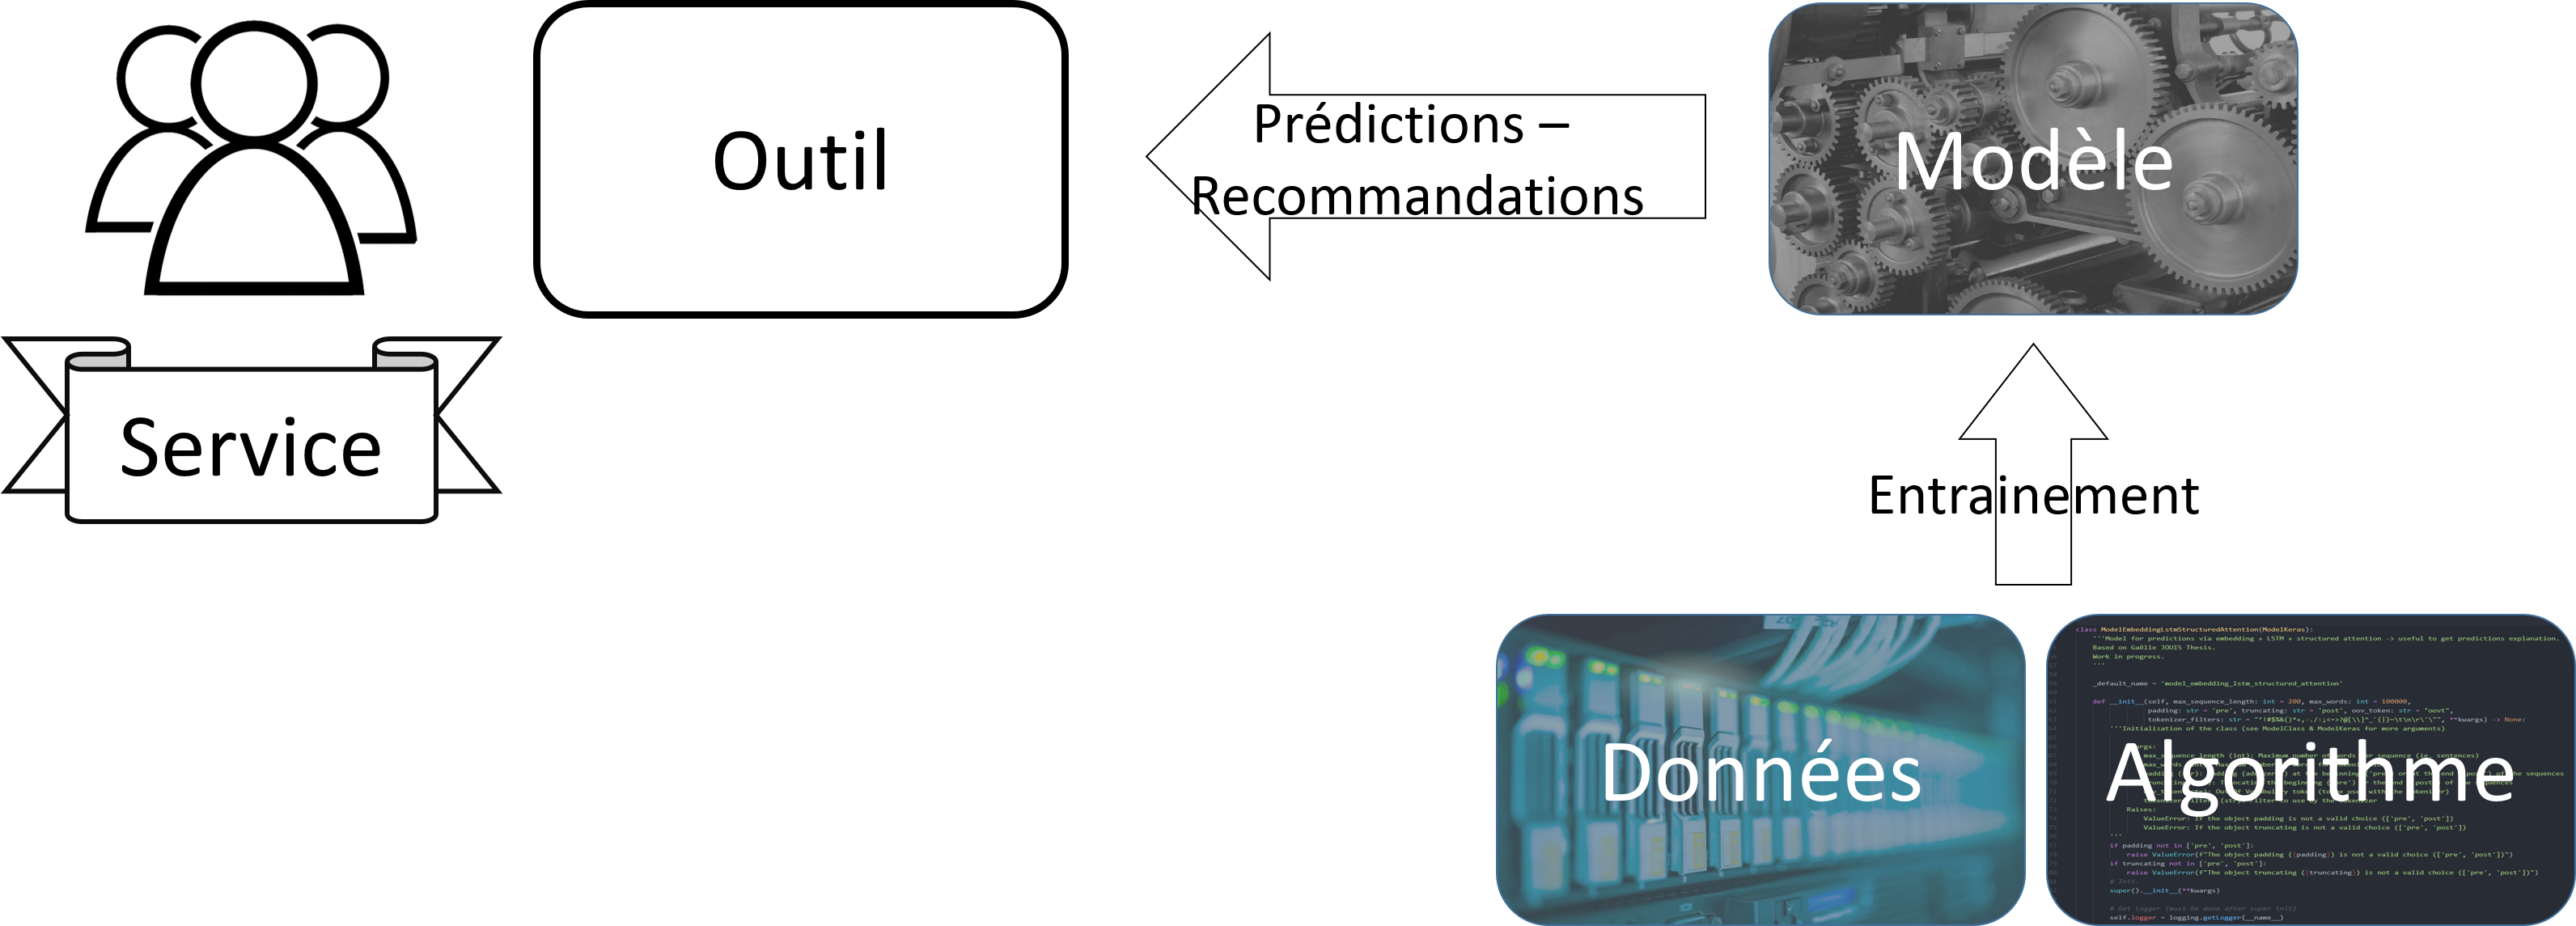
\includegraphics[width=\textwidth]{Introduction/figures/environnement.png}
    \caption{L'environnement des travaux. Des utilisateurs veulent bénéficier d'un service. Iels utilisent un outil qui présente les prédictions d'un modèle. Le modèle est lui même entraîné à partir d'un algorithme et de données.}
    \label{fig:environnement}
\end{figure}

% explicabilité
Nous proposons des explications permettant à l’utilisateur de comprendre les résultats obtenus et le modèle. Ces explications sont présentées sous forme d'interfaces.
% Des modèles profonds
Les modèles cibles sont les plus complexes: les réseaux de neurones profonds.
% Sur des données textuelles
Nous nous concentrons spécifiquement sur les architectures d'analyse de textes et sur des visualisations prenant en compte les spécificités du langage naturel.
% Pour Pôle emploi
Ces travaux sont intégrés à un outil commun aux scientifiques des données de Pôle emploi, et accessibles en open source.

Notre contribution est donc constituée des éléments suivants :
\begin{itemize}
    \item La création d'un jeu de données de classification de textes avec les explications locales associées,
    \item L'application de deux méthodes de génération d'explication locales de la littérature : les ancres et le mécanisme d'attention,
    \item La définition d'un protocole de comparaison de ces explications, avec et sans utilisateurs,
    \item Un démonstrateur permettant de présenter des interfaces adaptées aux utilisateurs, interfaces définies grâce à un test d'utilisabilité réalisé directement auprès des utilisateurs,
    \item Une méthode modulaire de génération d'explications globales, via l'aide à la création d'un modèle mental par les utilisateurs.
\end{itemize}

\section*{Plan}
\addcontentsline{toc}{section}{Plan}
% 1 page : toute l'histoire du manuscrit

% C1 : état de l'art
Dans le chapitre 1 nous nous intéresserons à la littérature du domaine. Cet état de l'art commence par la définition des méthodes d'explications et présente la diversité des explications possibles. Ensuite nous abordons les méthodes de génération d'explications, et leur évaluation.

% C2 : prérequis - données, démonstrateur, génération d'explications locales
Ensuite, dans le chapitre 2 nous présentons les pré-requis à nos travaux, à savoir la collecte et définition d'un jeu de données d'explications de référence. Nous appliquons deux méthodes de génération d'explications locales issues de l'état de l'art à nos données de référence. Enfin, nous présentons notre démonstrateur, permettant la visualisation de ces explications locales.

% C3 : protocoles d'évaluation et comparaison d'explications locales avec et sans utilisateurs
Le chapitre 3 définit le protocole de comparaison d'explications locales. Dans un premier temps nous évaluons la forme des explications grâce à un test d'utilisabilité auprès d'un panel restreint d'utilisateurs. Nous évaluons ensuite le contenu des explications. Deux contextes majeurs sont pris en compte : la présence ou absence d'utilisateurs experts disponibles.

% C4 : Méthode modulaire d'explications globales
Dans le chapitre 4 nous introduisons une méthode modulaire d'explication globale d'un modèle, par l'aide à la définition d'un modèle mental pour l'utilisateur. Nous implémentons une stratégie avec un effort de réduction des calculs nécessaires. L'application sur nos données réelles permet de prouver son potentiel et d'en déterminer les limites.

% C5 : Intégration des travaux à leur environnement industriel
Enfin, nous mettons en avant dans le chapitre 5 le lien fort entre les travaux effectués et leur contexte industriel. Nous présentons le cadre logiciel de développement de Pôle Emploi, auquel sont ajoutées les fonctionnalités d'explications locales et globales présentées. La charte éthique de l'établissement est présentée ainsi que l'intégration de nos travaux à sa mise en œuvre. Enfin, nous proposons une ébauche de guides destinés aux industriels, notamment gestionnaires de projets, leur permettant de mieux définir leurs besoins en explicabilité, et les méthodes de la littérature qui seraient les mieux adaptées à ces besoins.

% comment générer une explication : donne \cite{Jouis2020}
